\documentclass[crop,tikz]{standalone}

\begin{document}

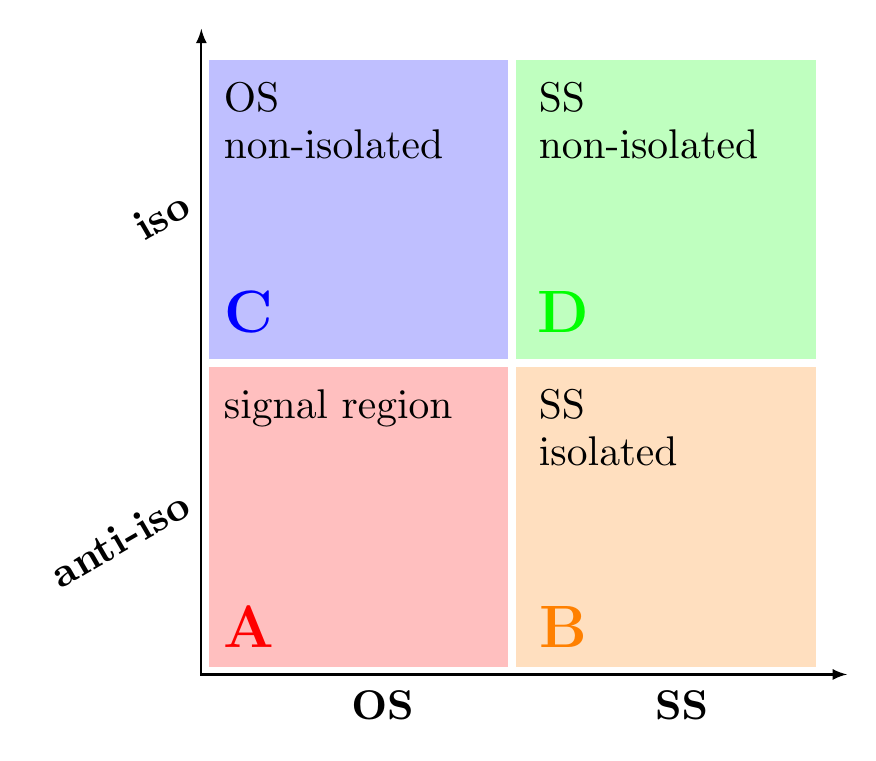
\begin{tikzpicture}[scale=2, every node/.style={scale=1.5}]
  \def\amax{4.1} % x axis maximum
  \def\opac{0.25} % opacity
  
  % AXES
  \draw[<->,>=latex,thick] (\amax,0) node[below left] {$$}
  -| (0,\amax) node[above left,rotate=90] {};

  \fill [red, opacity=\opac]    (0.05,0.05) rectangle (1.95,1.95);
  \fill [orange, opacity=\opac] (2.0,0.05)  rectangle (3.9,1.95);
  \fill [blue, opacity=\opac]   (0.05,2.0)  rectangle (1.95,3.9);
  \fill [green, opacity=\opac]  (2.0,2.0)   rectangle (3.9,3.9);
  
  \node [red]    at (0.3,0.3) {\Large \textbf{A}};
  \node [orange] at (2.3,0.3) {\Large \textbf{B}};
  \node [blue]   at (0.3,2.3) {\Large \textbf{C}};
  \node [green]  at (2.3,2.3) {\Large \textbf{D}};

  \node [black, anchor = north west] at (0.05,1.9) {signal region};
  \node [black, anchor = north west] at (2.05,1.9) {SS};
  \node [black, anchor = north west] at (2.05,1.6) {isolated};
  \node [black, anchor = north west] at (0.05,3.85) {OS};
  \node [black, anchor = north west] at (0.05,3.55) {non-isolated};
  \node [black, anchor = north west] at (2.05,3.85) {SS};
  \node [black, anchor = north west] at (2.05,3.55) {non-isolated};

  \node [black, rotate=30, anchor = east] at (-0.02,3.05) {\textbf{iso}};
  \node [black, rotate=30, anchor = east] at (-0.02,1.15) {\textbf{anti-iso}};
  \node [black, anchor = north] at (1.15,-0.01) {\textbf{OS}};
  \node [black, anchor = north] at (3.05,-0.01) {\textbf{SS}};

\end{tikzpicture}

\end{document}
